% Pengaturan ukuran teks dan bentuk halaman dua sisi
\documentclass[12pt]{book}

% Pengaturan ukuran halaman dan margin
\usepackage[a4paper,top=30mm,left=30mm,right=20mm,bottom=25mm]{geometry}

% Pengaturan ukuran spasi
\usepackage[singlespacing]{setspace}

% Pengaturan caption untuk tabel
\usepackage{caption}

% Judul dokumen
\title{Proposal Tugas Akhir ITS}
\author{Cisatra, Aulia}

% Pengaturan detail pada file PDF
\usepackage[pdfauthor={\@author},bookmarksnumbered,pdfborder={0 0 0}]{hyperref}


% Pengaturan ukuran indentasi
\setlength{\parindent}{2em}

% Package lainnya
\usepackage{changepage}
\usepackage{etoolbox} % Mengubah fungsi default

% Pengaturan jenis karakter
\usepackage[utf8]{inputenc}

\usepackage[style=apa, backend=biber]{biblatex}
\usepackage{enumitem} % Pembuatan list
\usepackage{lipsum} % Pembuatan template kalimat
\usepackage{graphicx} % Input gambar
\usepackage{longtable} % Pembuatan tabel
\usepackage[table,xcdraw]{xcolor} % Pewarnaan tabel
\usepackage{eso-pic} % Untuk menggunakan background image di halaman
\usepackage{txfonts} % Font times
\usepackage{changepage} % Pembuatan teks kolom
\usepackage{multicol} % Pembuatan kolom ganda
\usepackage{multirow} % Pembuatan baris ganda
\usepackage{tabularx} % Untuk mengatur kolom, seperti grid pada CSS
\usepackage{wrapfig}
\usepackage{float}

% Pengaturan format daftar isi, daftar gambar, dan daftar tabel
\usepackage[titles]{tocloft}
\setlength{\cftsecindent}{2em}
\setlength{\cftsubsecindent}{2em}
\setlength{\cftbeforechapskip}{1.5ex}
\setlength{\cftbeforesecskip}{1.5ex}
\setlength{\cftbeforetoctitleskip}{0cm}
\setlength{\cftbeforeloftitleskip}{0cm}
\setlength{\cftbeforelottitleskip}{0cm}
\renewcommand{\cfttoctitlefont}{\hfill\Large\bfseries} % command untuk membuat heading bold dan besar
\renewcommand{\cftaftertoctitle}{\hfill}
\renewcommand{\cftloftitlefont}{\hfill\Large\bfseries}
\renewcommand{\cftafterloftitle}{\hfill}
\renewcommand{\cftlottitlefont}{\hfill\Large\bfseries}
\renewcommand{\cftafterlottitle}{\hfill}

% Definisi untuk "Hati ini sengaja dikosongkan"
\patchcmd{\cleardoublepage}{\hbox{}}{
  \thispagestyle{empty}
  \vspace*{\fill}
  \begin{center}\textit{[Halaman ini sengaja dikosongkan]}\end{center}
  \vfill}{}{}

  % Pengaturan penomoran halaman
\usepackage{fancyhdr}
\fancyhf{}
\renewcommand{\headrulewidth}{0pt}
\pagestyle{fancy}
\fancyfoot[C,CO]{\thepage}
\patchcmd{\chapter}{plain}{fancy}{}{}
\patchcmd{\chapter}{empty}{plain}{}{}

% Pengaturan format judul bab
\usepackage{titlesec}
\renewcommand{\thesection}{\thechapter.\arabic{section}}
\titleformat{\chapter}[hang]{\centering\bfseries\large}{BAB\ \arabic{chapter}\ }{0ex}{\vspace{0ex}\centering}
\titleformat*{\section}{\large\bfseries}
\titleformat*{\subsection}{\normalsize\bfseries}
\titlespacing{\chapter}{0ex}{0ex}{4ex}
\titlespacing{\section}{0ex}{1ex}{0ex}
\titlespacing{\subsection}{0ex}{0.5ex}{0ex}
\titlespacing{\subsubsection}{0ex}{0.5ex}{0ex}
\setcounter{secnumdepth}{3} % Untuk memberi penomoran pada \subsubsection

\counterwithin{figure}{chapter}
\counterwithin{table}{chapter}

% Mengganti figure dan table menjadi gambar dan tabel
\renewcommand{\figurename}{Gambar}
\renewcommand{\tablename}{Tabel}

% Tambahkan format tanda hubung yang benar di sini
\hyphenation{
  ro-ket
  me-ngem-bang-kan
  per-hi-tu-ngan
}

% Menambahkan resource daftar pustaka
\addbibresource{pustaka/pustaka.bib}

% Isi keseluruhan dokumen
\begin{document}
  % Nomor halaman pembuka dimulai dari sini
  \pagenumbering{roman}

  % Atur ulang penomoran halaman
  \setcounter{page}{1}

  % Sampul Bahasa Indonesia
  \newcommand\covercontents{sampul/konten-id.tex}
  \AddToShipoutPictureBG*{
  \AtPageLowerLeft{
    % Ubah nilai berikut jika posisi horizontal background tidak sesuai
    \hspace{-3.25mm}

    % Ubah nilai berikut jika posisi vertikal background tidak sesuai
    \raisebox{0mm}{
      
\includegraphics[width=\paperwidth,height=\paperheight]{sampul/gambar/sampul-luar-tipis.png}
    }
  }
}

% Menyembunyikan nomor halaman
\thispagestyle{empty}

% Pengaturan margin untuk menyesuaikan konten sampul
\newgeometry{
  top=65mm,
  left=30mm,
  right=30mm,
  bottom=20mm
}

\begin{flushleft}

  % Pemilihan font sans serif
  \sffamily

  % Pemilihan font bold
  \fontseries{bx}
  \selectfont
  \begin{spacing}{1.5}
    \input{\covercontents}
  \end{spacing}

\end{flushleft}

\restoregeometry


  % Lembar pengesahan
  \chapter*{LEMBAR PENGESAHAN}

% Menyembunyikan nomor halaman
\thispagestyle{empty}

\begin{center}
  % Ubah kalimat berikut dengan judul tugas akhir
  \textbf{KALKULASI ENERGI PADA ROKET LUAR ANGKASA BERBASIS \emph{ANTI-GRAVITASI}}
\end{center}

\begingroup
% Pemilihan font ukuran small
\small

\begin{center}
  % Ubah kalimat berikut dengan pernyataan untuk lembar pengesahan
  \textbf{PROPOSAL TUGAS AKHIR} \\
  Diajukan untuk memenuhi salah satu syarat memperoleh gelar
  Sarjana Teknik pada
  Program Studi S-1 Teknik Dirgantara \\
  Departemen Teknik Dirgantara \\
  Fakultas Teknik Dirgantara \\
  Institut Teknologi Sepuluh Nopember
\end{center}

\begin{center}
  % Ubah kalimat berikut dengan nama dan NRP mahasiswa
  Oleh: \textbf{Elon Reeve Musk} \\
  NRP. 0123 20 4000 0001
\end{center}

\begin{center}
  Disetujui Oleh:
\end{center}

\vspace{10ex}

\begingroup
% Menghilangkan padding
\setlength{\tabcolsep}{0pt}

\noindent
\begin{tabularx}{\textwidth}{X c}
  % Ubah kalimat-kalimat berikut dengan nama dan NIP dosen pembimbing pertama
  Nikola Tesla, S.T., M.T.      &                 \\
  NIP: 18560710 194301 1 001    & (Pembimbing)    \\
                                &                 \\
                                &                 \\
                                &                 \\
  % Ubah kalimat-kalimat berikut dengan nama dan NIP dosen pembimbing kedua
  Wernher von Braun, S.T., M.T. &                 \\
  NIP: 19230323 197706 1 001    & (Ko-Pembimbing) \\
\end{tabularx}
\endgroup

\vspace{\fill}

\begin{center}
  % Ubah text dibawah menjadi tempat dan tanggal
  \textbf{SURABAYA} \\
  \textbf{Mei, 2077}
\end{center}
\endgroup

  \cleardoublepage

  % Abstrak
  \chapter*{ABSTRAK}
\begin{center}
  \large
  \textbf{KALKULASI ENERGI PADA ROKET LUAR ANGKASA BERBASIS \emph{ANTI-GRAVITASI}}
\end{center}
\addcontentsline{toc}{chapter}{ABSTRAK}
% Menyembunyikan nomor halaman
\thispagestyle{empty}

\begin{flushleft}
  \setlength{\tabcolsep}{0pt}
  \bfseries
  \begin{tabular}{ll@{\hspace{6pt}}l}
  Nama Mahasiswa / NRP&:& Elon Reeve Musk / 0123204000001\\
  Departemen&:& Teknik Dirgantara FTD - ITS\\
  Dosen Pembimbing&:& 1. Nikola Tesla, S.T., M.T.\\
  & & 2. Wernher von Braun, S.T., M.T.\\
  \end{tabular}
  \vspace{4ex}
\end{flushleft}
\textbf{Abstrak}

% Isi Abstrak
Abstrak harus berisi seratus hingga dua ratus kata. \lipsum[1]

\vspace{2ex}
\noindent
\textbf{Kata Kunci: \emph{Roket, Anti-gravitasi, Meong}}
  \cleardoublepage

  \chapter*{ABSTRACT}
\begin{center}
  \large
  \textbf{\emph{ANTI-GRAVITY} BASED ENERGY CALCULATION ON OUTER SPACE ROCKETS}
\end{center}
% Menyembunyikan nomor halaman
\thispagestyle{empty}

\begin{flushleft}
  \setlength{\tabcolsep}{0pt}
  \bfseries
  \begin{tabular}{lc@{\hspace{6pt}}l}
  Student Name / NRP&: &Elon Reeve Musk / 0123204000001\\
  Department&: &Aerospace Engineering FTD - ITS\\
  Advisor&: &1. Nikola Tesla, S.T., M.T.\\
  & & 2. Wernher von Braun, S.T., M.T.\\
  \end{tabular}
  \vspace{4ex}
\end{flushleft}
\textbf{Abstract}

% Isi Abstrak
The abstract must consist between two hundred to three hundred words. \lipsum[1]

\vspace{2ex}
\noindent
\textbf{Keywords: \emph{Rocket, Anti-gravity, Meong}}
  \cleardoublepage

  \begin{spacing}{1.5}
    % Daftar isi
    \renewcommand*\contentsname{DAFTAR ISI}
    \addcontentsline{toc}{chapter}{\contentsname}
    \tableofcontents
    \cleardoublepage

    % Daftar gambar
    \renewcommand*\listfigurename{DAFTAR GAMBAR}
    \addcontentsline{toc}{chapter}{\listfigurename}
    \listoffigures
    \cleardoublepage

    % Daftar tabel
    \renewcommand*\listtablename{DAFTAR TABEL}
    \addcontentsline{toc}{chapter}{\listtablename}
    \listoftables
    \cleardoublepage
  \end{spacing}

  % Nomor halaman isi dimulai dari sini
  \pagenumbering{arabic}

  % Konten pendahuluan
  \chapter{PENDAHULUAN}

\section{Latar Belakang}
Dashboard kinerja adalah salah satu alat teknologi yang dapat membantu memberikan informasi bagi manajemen rumah sakit untuk melakukan pengambilan keputusan. Dengan kemajuan teknologi informasi dalam industri kesehatan, penggunaan dashboard kinerja telah menjadi semakin penting. Berdasarkan penelitian milik Luigi Jesus Basile, pemanfaatan dashboard kinerja dan \emph{Business Intelligence} (BI) dalam pengambilan keputusan dapat mengungguli praktik berbasis pengalaman dalam mengelola proses di sektor kesehatan \parencite{Basile2023}. Selain itu, laporan yang dikeluarkan oleh Capital link terkait \emph{Performance Benchmarking Toolkit for Health Centers} menjelaskan bahwa penerapan alat analis data membantu pemimpin dalam melacak kinerja secara lebih efektif dan efisien, memahami faktor utama yang memengaruhi, serta menggabungkan pemahaman tentang operasional untuk menjadikan pusat kesehatan lebih berkelanjutan secara finansial dan mencapai kesuksesan yang berkelanjutan \parencite{CapitalLink2017}. Implementasi dashboard kinerja menjadi lebih mendesak dalam berbagai situasi kesehatan yang memerlukan pemantauan real-time dan analisis data untuk membantu manajemen rumah sakit merespons dengan lebih cepat dan tepat.


Dalam penerapan dashboard kinerja di lingkungan rumah sakit, pengumpulan dan integrasi data menjadi komponen kunci. Integrasi data adalah proses menggabungkan data dari berbagai sumber yang berbeda menjadi satu kesatuan yang terintegrasi \parencite{Neang2021DataIA}. Data yang diperlukan untuk menghasilkan wawasan yang komprehensif dan bermakna dalam operasional rumah sakit bersumber dari berbagai proses bisnis yang terjadi di lingkungan rumah sakit. Data tersebut termasuk data pasien yang mencakup data pendaftaran atau data rawat inap;informasi dokter yang melibatkan jadwal praktek;persediaan obat-obatan yang mencakup inventaris obat dan alas medis;serta berbagai elemen lainnya seperti administrasi, keuangan, dan manajemen sumber daya manusia.


Berdasarkan data yang dihimpun oleh Pusat Kedokteran dan Kesehatan (Pusdokkes) polri, saat ini terdapat 57 cabang rumah sakit polri yang tersebar di berbagai daerah \parencite{Aziz2023OptimalisasiPD}. Setiap cabang rumah sakit melakukan proses bisnis yang sama, yaitu melayani masyarakat dalam hal kesehatan. Dengan kegiatan layanan kesehatan yang dilakukan setiap hari, tentunya jumlah data untuk setiap cabang rumah sakit akan terus bertambah. Proses integrasi data menjadi semakin penting dalam konteks ini, karena akan memungkinkan manajemen pusat rumah sakit polri untuk melakukan analisis kualitas pelayanan kesehatan baik pada setiap cabang ataupun keseluruhan cabang dengan lebih efisien.


Namun, meskipun pentingnya pengumpulan dan integrasi data ini sangat jelas, kenyataannya mengungkapkan tantangan serius. Berdasarkan wawancara dengan salah satu developer dari simkes Khanza, saat ini setiap cabang rumah sakit masih mengoprasikan sistem infomasi yang terpisah-pisah dan dijalankan secara lokal. Dampak dari hal ini adalah basis data dari setiap cabang rumah sakit belum terintegrasi dengan basis data sentral. Basis data sentral tersebut diharapkan terhubung dengan dashboard kinerja guna memantau kinerja baik keseluruhan cabang ataupun satu-persatu. Ketidaktersediaan integrasi data tersebut menjadi hambatan signifikan dalam upaya membangun dan mengimplementasikan dashboard kinerja yang efektif. Untuk mengatasi hambatan ini, perlu ditemukan solusi yang memungkinkan pengumpulan dan integrasi data dari berbagai cabang rumah sakit, sehingga dashboard kinerja dapat memberikan manfaat maksimal dalam mengingkatkan kualitas dan efisiensi layanan kesehatan.\parencite{Basile2023}

Beberapa upaya mengenai integrasi data sudah pernah dilakukan oleh \textcite{Firdaus2022MEMBANGUNID} berupa implementasi desain ETL (Extract-Transform-Load) yang dapat mengolah data dari berbagai sumber dengan menggunakan Microsoft SSIS (SQL Server Integration Service) untuk merancang aliran data dari sumber ke basis data tujuan. Meskipun upaya ini memiliki manfaat signifikan dalam menyatukan data dari berbagai sumber, terdapat kelemahan yang perlu diperhatikan. Salah satu kelemahan yang terjadi pada penelitian ini adalah penggunaan perangkat lunak pihak ketiga yang membatasi pengguna harus menggunakan basis data tertentu sebagai basis data tujuan. Penggunaan alat tertentu dapat menghambat proses integrasi disebabkan tidak kompatibelnya alat tersebut dengan infrastruktur rumah sakit.


Penelitian lain terkait integrasi data telah dilakukan oleh \textcite{Herfandi_Julkarnain_Hanif_2022}, yang mengimplementasikan RESTful Application Programming Interface (API) sebagai penghubung antara dua aplikasi pencatatan data untuk mencapai integrasi. Penelitian ini memiliki pendekatan yang berbeda, di mana tidak ada perpindahan data yang terjadi, melainkan hanya penggabungan akses pada dua basis data dalam satu aplikasi. Salah satu kelemahan yang dapat diidentifikasi pada penelitian ini adalah ketergantungan pada sumber data yang sudah harus tersedia di \emph{cloud} agar dapat diakses melalui internet. Hal ini menjadi masalah karena dalam konteks sistem informasi rumah sakit, banyak rumah sakit masih menerapkan sistem secara lokal karena kekhawatiran akan aspek keamanan data. 

Upaya yang telah diuraikan berdasarkan penelitian-penelitian sebelumnya masih belum mampu untuk menjadi solusi terhadap permasalahan integritas data pada sistem informasi rumah sakit. Terlebih lagi proses migrasi data menjadi lebih rumit disebabkan heterogenitas data pada sistem informasi rumah sakit. Sebagaimana yang telah dijelaskan oleh penelitian yang dilakukan oleh \textcite{Elamparithi2015}, migrasi data dapat menjadi tugas yang memakan waktu dan sangat mahal berbanding lurus dengan kekompleksan data; oleh karena itu, organisasi perlu menyederhanakan proses migrasi dan menjadikannya semaksimal mungkin dalam hal efisiensi biaya. Selain itu ancaman kebocoran data juga menjadi hal yang perlu diperhatikan selama proses migrasi data. Data dari Ponemon Institute dalam laporan \emph{Cost of a Data Breach Report 2023} mengungkapkan bahwa biaya kebocoran data di sektor kesehatan dapat mencapai rata-rata \$11 juta \parencite{Ponemon2023}. Hal ini menggarisbawahi pentingnya menjaga keamanan data selama proses migrasi data, yang dapat menjadi sangat kompleks dan rentan terhadap serangan siber.


Dari permasalahan yang telah diuraikan di atas, diperlukan suatu perangkat lunak yang dapat mengintegrasikan basis data dari setiap cabang rumah sakit ke basis data sentral
yang terhubung dengan dashboard kinerja dengan mempertimbangkan kekompleksan data pada sistem informasi rumah sakit. Perangkat lunak tersebut fokus pada perpindahan data pada basis data lokal sistem informasi rumah sakit dan juga meminimalkan risiko keamanan data yang dapat terjadi ketika proses perpindahan data. Selain itu perangkat lunak juga mempunyai fleksibitas dalam hal menerima data dari berbagai sumber basis data dan juga memindahkan data ke basis data sentral yang telah ditentukan.

\clearpage

\section{Rumusan Masalah}
Berdasarkan hal yang telah dipaparkan di latar belakang, maka dapat dirumuskan masalah sebagai berikut:
\begin{enumerate}
    \item bagaimana merancang dan membangun perangkat lunak integrasi data yang efektif untuk mengintegrasikan data dari setiap cabang rumah sakit ke basis data sentral?
    \item bagaimana merancang dan membangun perangkat lunak integrasi data yang meminimalkan risiko keamanan data selama proses integrasi?
    \item bagaimana merancang dan membangun perangkat lunak integrasi data yang memiliki fleksibilitas dalam menerima data dari berbagai sumber basis data dan memindahkan data ke basis data sentral yang telah ditentukan?
\end{enumerate}

\section{Batasan Masalah atau Ruang Lingkup}
Berdasarkan latar belakang dan rumusan masalah, maka dapat dirumuskan batasan masalah sebagai berikut:
\begin{enumerate}
    \item perangkat lunak integrasi data hanya dapat mengintegrasikan data dari sumber sistem basis data SQl seperti MySQL, PostgreSQL dan MSSQL;
    \item perangkat lunak integrasi data hanya dijalankan pada perangkat yang memiliki sistem operasi Windows; dan
    \item perangkat lunak integrasi data hanya dapat dijalankan menggunakan jaringan yang terhubung dengan server yang menyimpan basis data sistem informasi rumah sakit.
\end{enumerate}

\section{Tujuan}
Berdasarkan rumusan masalah dan batasan masalah, maka dapat dirumuskan tujuan sebagai berikut:
\begin{enumerate}
    \item merancang dan membangun perangkat lunak integrasi data yang efektif untuk mengintegrasikan data dari setiap cabang rumah sakit ke basis data sentral;
    \item merancang dan membangun perangkat lunak integrasi data yang meminimalkan risiko keamanan data selama proses integrasi; dan
    \item merancang dan membangun perangkat lunak integrasi data yang memiliki fleksibilitas dalam menerima data dari berbagai sumber basis data dan memindahkan data ke basis data sentral yang telah ditentukan.
\end{enumerate}

\section{Manfaat}
Berikut adalah manfaat yang diharapkan dari Tugas Akhir yang dilakukan:
\begin{enumerate}
    \item Memberikan kontribusi bagi rumah sakit Bhayangkara dalam meningkatkan efisiensi operasional dan meningkatkan pelayanan kesehatan bagi pasien.
    \item Memberikan kontribusi bagi peneliti selanjutnya dalam melakukan penelitian terkait sistem integrasi data.
\end{enumerate}


  \cleardoublepage

  % Konten tinjauan pustaka
  \chapter{TINJAUAN PUSTAKA}

% Ubah konten-konten berikut sesuai dengan isi dari tinjauan pustaka
\section{Hasil penelitian/perancangan terdahulu}
Proposal Tugas Akhir ini disusun berdasarkan beberapa hasil penelitian terdahulu dengan perincian sebagai berikut:
\renewcommand\tabularxcolumn[1]{m{#1}}
\begin{table}[ht]
  \caption{Table penelitian perangkat lunak integrasi data pada fasilitas kesehatan}
  \label{tab:penelitian-terdahulu}
  \centering
  \begin{tabularx}{\textwidth}{|p{3.5cm}|X|}
    \hline
    \textbf{Judul Penelitian} & A data integration platform for patient-centered e-healthcare and clinical decision support \\
    \hline
    \textbf{Peneliti dan Tahun terbit} & Jayaratne, Madhura;Nallaperuma, Dinithi;De Silva, Daswin;Alahakoon, Damminda;Devitt, Brian;Webster, Kate E.;Chilamkurti, Naveen.2019. \\
    \hline
    \textbf{Rangkuman Penelitian} & Artikel ini menjelaskan solusi teknis untuk penyampaian layanan kesehatan berkualitas tinggi dengan mengusulkan sebuah platform untuk mengintegrasikan data dan informasi mengenai hubungan yang terjalin antara profesional kesehatan, pasien, dan pengasuh mereka. Sistem yang diusulkan bertujuan untuk memberikan perawatan yang disesuaikan dengan individu bagi para pasien dengan mematuhi teori IS yang diusulkan. Sistem ini mengatasi masalah-masalah seperti heterogenitas data dan integrasi data berbasis pasien. Artikel ini menyimpulkan bahwa platform yang diusulkan dapat dianggap sebagai langkah besar menuju pencapaian perawatan berbasis pasien (PCC) di berbagai praktik medis, baik yang kecil maupun besar.\\
    \hline
    \textbf{Keterkaitan Penelitian} & Pada penelitian ini dijelaskan terkait kompleksitas data pada layanan kesehatan. Kompleksitas data terdapat heterogenitas data pasien yang berbeda dari berbagai segi. Ketekaitan dengan penelitian ini adalah pertama kesamaan studi kasus yang dipilih yaitu integritas data pada layanan kesehatan dan juga permasalahan terkait komplesitas data akibat heterogenitas data. \\
    \hline
  \end{tabularx}
\end{table}

\clearpage

\begin{table}[ht]
  \caption{Table penelitian perangkat lunak integrasi data dengan metode ETL}
  \label{tab:penelitian-terdahulu-2}
  \centering
  \begin{tabularx}{\textwidth}{|p{3.5cm}|X|}
    \hline
    \textbf{Judul Penelitian} & Pengembangan Dashboard Cerdas Untuk Monitoring Data Pasien Rawat Rumah Sakit Umum Daerah Praya Kabupaten Lombok Tengah \\
    \hline
    \textbf{Peneliti dan Tahun terbit} & Mutawalli; Lalu; Zaen; Asri; Bagye, Wire.2021. \\
    \hline
    \textbf{Rangkuman Penelitian} & Artikel ini membahas pengembangan data warehouse dan dashboard untuk mengintegrasikan data antara dua Hospital Information System (SIM RS) di RSUD Praya. Dashboard ini bertujuan untuk membantu rumah sakit dalam mengeluarkan informasi dari dataset, seperti analisis metode pembayaran, jenis penyakit, dan membandingkan jumlah pasien dengan gender yang berbeda, dari data inpatient. Dashboard ini juga digunakan untuk menentukan distribusi dan asal seorang pasien. Pengujian sistem dilakukan melalui pengujian langsung pengguna, hasilnya menunjukkan skor dashboard sistem sebesar 86\%, mencakup kualitas sistem pada 86\%, kualitas informasi pada 88\%, dan kualitas layanan pada 85\%. Kesimpulan dari penelitian ini menunjukkan bahwa sistem cukup mendukung kinerja pemangku kepentingan di rumah sakit publik regional di Praya.\\
    \hline
    \textbf{Keterkaitan Penelitian} & Pada penelitian ini digunakan metode ETL dalam proses integrasi data antara dua rumah sakit. Walaupun proses ETL dilakukan dengan menggunakan aplikasi pihak ketiga, namun proses yang dijelaskan cukup untuk memberikan referensi terhadap penelitian ini \\
    \hline
  \end{tabularx}
\end{table}

\clearpage

\section{Teori/Konsep Dasar}

\subsection{Integrasi Data}
Integrasi data adalah proses menggabungkan data dari berbagai sumber menjadi tampilan yang terpadu \parencite{Neang2021DataIA}. Dalam konteks rumah sakit, data dari berbagai sumber seperti catatan medis, informasi pasien, pengelolaan inventaris, keuangan, dan departemen lainnya perlu disatukan secara holistik \parencite*{Oliva2018}. Proses integrasi data ini penting karena memungkinkan penyedia layanan kesehatan dan staf administratif mengakses informasi yang konsisten dan terintegrasi, memfasilitasi pengambilan keputusan yang lebih cepat dan akurat \parencite{Basile2023}. Dalam Penerapan integrasi data, terdapat beberapa penelitian yang menggunakan berbagai metode yang berbeda. Penelitian oleh \textcite{Baharuddin2022IMPLEMENTASIWS} menerapkan metode RESTful Web Services sebagai alat integrasi data. Dengan metode tersebut memungkinkan aplikasi untuk mengakses data dari database lain melalui API. Sedangkan penelitian oleh \textcite{Firdaus2022MEMBANGUNID} menerapkan metode ETL dalam proses integrasi data. Metode Restful API memiliki keunggulan dalam kecepatan mengakses data namun pada akhirnya data yang diakses tersebut tidak dipindahkan ke database baru namun hanya diakses saja, sedangkan metode ETL melibatkan perpindahan data yang menyebabkan proses menjadi lebih rumit dan memerlukan banyak waktu dan tenaga. Adapun tantangan dalam integrasi data melibatkan beberapa aspek krusial antara lain,
\begin{enumerate}
  \item Kesulitan dalam menggabungkan data dari berbagai sumber yang berbeda.
  \item Memastikan keakuratan dan konsistensi data yang diintegrasikan.
  \item Menangani kompleksitas teknis dan keamanan dalam mengintegrasikan data dari berbagai platform.
\end{enumerate}


\subsection{Heterogeneous Data dalam Konteks Sistem Informasi Rumah Sakit}
Dalam konteks sistem informasi rumah sakit, heterogenitas data merujuk pada berbagai jenis dan sumber data serta format data yang digunakan pada sistem informasi rumah sakit. Heterogeneitas data tersebut mencakup data klinis dari berbagai departemen, seperti rekam medis pasien, informasi keuangan, dan data operasional yang berasal dari berbagai sumber, seperti sistem informasi manajemen rumah sakit (HIS), sistem informasi akuntansi, dan sistem informasi human resources \parencite{Amelia2021}. Aspek data klinis melibatkan detail-detail kompleks dari riwayat pasien, rencana perawatan, dan prosedur medis, sementara data keuangan berkaitan dengan catatan tagihan, klaim asuransi, dan informasi anggaran yang penting untuk mengelola operasi keuangan rumah sakit. Sementara itu, data operasional mencakup hal-hal seperti jadwal staf, alokasi sumber daya, dan manajemen inventaris, masing-masing berasal dari sistem-sistem terpisah yang melayani fungsionalitas khusus dalam rumah sakit \parencite{mutawalli2021pengembangan}.

\subsection{Metode ETL}
ETL merupakan singkatan dari Extract, Transform, Load, dan merupakan metode yang digunakan dalam data warehousing untuk mengumpulkan data dari berbagai sumber dan mengintegrasikannya menjadi satu data tunggal \parencite{Fana2021DataWD}. Proses ETL melibatkan tiga langkah utama \parencite{Peng2023}, yaitu:
\begin{enumerate}
  \item Ekstrak: Pada langkah ini, data diekstrak dari berbagai sumber, seperti basis data, berkas datar, atau layanan web.
  \item Transformasi: Data yang diekstrak kemudian diubah menjadi format yang dapat digunakan oleh gudang data. Ini mungkin melibatkan pembersihan data, penghapusan duplikat, atau konversi tipe data.
  \item Muat: Akhirnya, data yang telah diubah dimuat ke dalam basis data tujuan, di mana data tersebut dapat dianalisis dan digunakan untuk pelaporan serta pengambilan keputusan.
\end{enumerate}

ETL adalah proses penting dalam data warehousing, karena memastikan bahwa data di dalam gudang data akurat, konsisten, dan terkini. Terdapat faktor kunci yang memastikan kesuksesan proses ETL. Menurut \textcite{Ahmad2022THESF}, faktor-faktor utama yang berkontribusi pada kesuksesan proses ETL (Extract, Transform, Load) mencakup aspek kualitas sistem dan kualitas data. Faktor kualitas sistem menitikberatkan pada efisiensi dan kehandalan dari proses integrasi data, termasuk dalam hal kecepatan pemrosesan data, tingkat akurasi, dan konsistensi yang dijaga. Di sisi lain, faktor kualitas data mengacu pada kualitas dari data yang diintegrasikan, termasuk kelengkapan data, akurasi informasi, dan relevansi data dalam konteks integrasi tersebut. Kedua aspek ini memegang peran penting dalam memastikan kesuksesan dan kinerja yang optimal dari proses ETL.

\subsection{SQLite}
SQLite adalah sebuah c-languange library  yang mengimplementasikan sistem basis data SQL yang ringan dan cepat \parencite{sqlite-intro}. SQLite pada umumnya digunakan pada aplikasi dekstop atau embedded systems sebagai penyimpanan utama aplikasi. Dengan menggunakan SQLite, pengembang tidak perlu menginstall server atau melakukan konfigurasi sebelum menggunakan basis data ini. Adapun keunggulan dari basis data SQLite sebagai berikut \parencite{sqlite-advantage}.
\begin{enumerate}
  \item Mudah digunakan dan sederhana: SQLite mudah digunakan dan memerlukan minimal konfigurasi, sehingga cocok untuk aplikasi kecil dan sistem terintegrasi
  \item Self-contained: SQLite adalah database manajemen basa yang tidak memerlukan server dan dapat beroperasi tanpa dukungan jaringan. Ini membuatnya ideal untuk aplikasi yang membutuhkan operasi transaksi dan konsistensi tinggi.
  \item Kompatibilitas cross-platform: SQLite telah diportasi ke berbagai platform, termasuk Windows, macOS, dan iOS, membuatnya menjadi pilihan yang berversatil untuk aplikasi multi-platform
  \item Mendukung berbagai tipe data: SQLite mendukung full-text indexing dan JSON data, memungkinkan menyimpan dan mengolah data dalam berbagai format
\end{enumerate} 

\subsection{Electron JS}
Electron JS adalah kerangka kerja \emph{open-source} untuk membangun aplikasi desktop berbasis platform menggunakan teknologi web seperti HTML, CSS, dan Javascript \parencite{ElectronJS}. Dengan menggunakan Electron, pengembang dapat menciptakan aplikasi yang bekerja di berbagai platform, seperti macOS, Windows, dan Linux, dengan mengelola satu kode sumber JavaScript.

Keuntungan menggunakan Electron JS adalah pengembang dapat menggunakan teknologi web yang sudah dikuasai untuk membuat aplikasi desktop yang dapat berjalan di berbagai platform seperti Windows, macOS, dan Linux. Selain itu, Electron JS juga menyediakan akses ke API sistem operasi yang memungkinkan pengembang untuk mengakses fitur-fitur seperti notifikasi, sistem file, dan jaringan. Namun, karena aplikasi yang dibangun dengan Electron JS menggunakan teknologi web, aplikasi tersebut cenderung lebih berat dan memakan lebih banyak sumber daya dibandingkan dengan aplikasi desktop native \parencite{electonjs-alain}.

\subsection{Apache Beam}
Apache Beam merupakan suatu model pemrograman yang berfungsi untuk menentukan dan menjalankan serangkaian proses pemrosesan data, termasuk ETL (Ekstraksi, Transformasi, dan Pemuatan) pada batch dan stream processing \parencite{apacheoverview}. Dengan menggunakan SDK yang disediakan oleh Apache Beam, pengembang dapat mendefinisikan Beam Pipeline dan kemudian melakukan eksekusi pada runner (processing backend) yang didukung oleh Apache Beam seperti Apache Apex, Apache Flink, Apache Samza, Apache Spark, dan Google Cloud Dataflow \parencite{apacheoverview}.

Saat melakukan proses ETL, Apache Beam mempunyai konsep dasar seperti \emph{Pipeline} dan \emph{PCollection} yang merupakan kumpulan data yang akan diolah oleh Apache Beam. Selain itu, Apache Beam juga menawarkan kemampuan \emph{windowing} untuk membagi \emph{PCollection} berdasarkan waktu dari masing-masing elemennya, dan transformasi yang menggabungkan sejumlah elemen seperti GroupByKey. Apache Beam menggunakan \emph{trigger} untuk menetapkan waktu kapan hasil dari penggabungan akan dihasilkan untuk digunakan oleh langkah transformasi selanjutnya. Berdasarkan sumber \textcite{apache-advantage} Apache Beam memiliki beberapa keunggulan sebagai berikut.
\begin{enumerate}
  \item abstraksi yang kuat untuk memproses data pada batch dan streaming,
  \item menyediakan SDK yang dapat digunakan pada bahasa pemrograman,
  \item dapat membaca data dari berbagai sumber yang didukung, seperti Mysql, PostgreSQL, dll,
\end{enumerate}




% % Contoh pembuatan persamaan
% \begin{equation}
%   % Label referensi dari persamaan yang dibuat
%   \label{eq:FirstLaw}
%   % Baris kode persamaan yang dibuat
%   \sum \mathbf{F} = 0\; \Leftrightarrow\; \frac{\mathrm{d} \mathbf{v} }{\mathrm{d}t} = 0.
% \end{equation}

  \cleardoublepage

  % Konten metodologi
  \chapter{METODOLOGI}

% Ubah konten-konten berikut sesuai dengan isi dari metodologi

\section{Metode yang digunakan}

\lipsum[11]

% Contoh input gambar dengan format *.jpg
\begin{figure} [H] \centering
  % Nama dari file gambar yang diinputkan
  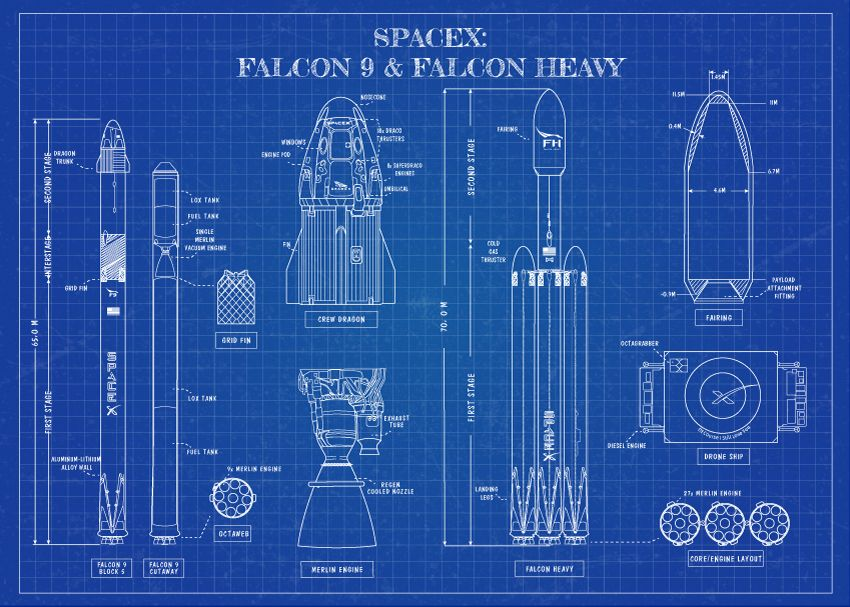
\includegraphics[scale=0.45]{gambar/blueprint.jpg}
  % Keterangan gambar yang diinputkan
  \caption{\emph{Blueprint} roket yang akan diuji coba \parencite{SpaceXBlueprint}}
  % Label referensi dari gambar yang diinputkan
  \label{fig:Blueprint}
\end{figure}

% Contoh penggunaan referensi dari gambar yang diinputkan
Pada \emph{blueprint} yang tertera di Gambar \ref{fig:Blueprint}. \lipsum[12]

\section{Bahan dan peralatan yang digunakan}

\lipsum[13]
\lipsum[3]

\section{Urutan pelaksanaan penelitian}

% Ubah tabel berikut sesuai dengan isi dari rencana kerja
\newcommand{\w}{}
\newcommand{\G}{\cellcolor{gray}}
\begin{table}[H]
  \captionof{table}{Tabel timeline}
  \label{tbl:timeline}
  \begin{tabular}{|p{3.5cm}|c|c|c|c|c|c|c|c|c|c|c|c|c|c|c|c|}

    \hline
    \multirow{2}{*}{Kegiatan} & \multicolumn{16}{|c|}{Minggu}                                                                       \\
    \cline{2-17}              &
    1                         & 2                             & 3  & 4  & 5  & 6  & 7  & 8  & 9  & 10 & 11 & 12 & 13 & 14 & 15 & 16 \\
    \hline

    % Gunakan \G untuk mengisi sel dan \w untuk mengosongkan sel
    Pengambilan data          &
    \G                        & \G                            & \G & \G & \w & \w & \w & \w & \w & \w & \w & \w & \w & \w & \w & \w \\
    \hline

    Pengolahan data           &
    \w                        & \w                            & \w & \w & \G & \G & \G & \G & \w & \w & \w & \w & \w & \w & \w & \w \\
    \hline

    Analisa data              &
    \w                        & \w                            & \w & \w & \w & \w & \w & \w & \G & \G & \G & \G & \w & \w & \w & \w \\
    \hline

    Evaluasi penelitian       &
    \w                        & \w                            & \w & \w & \w & \w & \w & \w & \w & \w & \w & \w & \G & \G & \G & \G \\
    \hline
  \end{tabular}
\end{table}

Pada \emph{timeline} yang tertera di Tabel \ref{tbl:timeline} \lipsum[10]

  \cleardoublepage

  % Konten lainnya
  \chapter{HASIL YANG DIHARAPKAN}

\section{Hasil yang Diharapkan dari Penelitian}

Dari penelitian yang akan dilakukan, diharapkan \lipsum[15]

\section{Hasil Pendahuluan}

Sampai saat ini, kami telah \lipsum[16]

  \cleardoublepage

  % Daftar pustaka
  \chapter*{DAFTAR PUSTAKA}
  \addcontentsline{toc}{chapter}{DAFTAR PUSTAKA}
  \renewcommand\refname{}
  \vspace{2ex}
  \renewcommand{\bibname}{}
  \begingroup
    \def\chapter*#1{}
    \printbibliography
  \endgroup


\end{document}
